\documentclass{beamer}
\usetheme{Madrid}
\usecolortheme{beaver}
\setbeamertemplate{navigation symbols}{}
\usepackage{tikz}
\usepackage{listings}
\usepackage{hyperref}
\usetikzlibrary{positioning, calc}


\title{System and Network Architecture in Security Operations}
\author{Brendan Shea, PhD}

\date{\today}

\begin{document}
	
	\begin{frame}
		\titlepage
	\end{frame}
	
	\begin{frame}
		\frametitle{1. Security Architecture: The Foundation of Modern Cybersecurity Operations}
		\begin{itemize}
			\item Security architecture provides the framework for implementing protective measures across systems and networks.
			\item \textbf{Security architecture} is defined as the design of systems and processes that protect information assets from unauthorized access or damage.
			\item Effective security architecture aligns with business goals while mitigating risks through defense-in-depth strategies.
			\item Security operations depend on well-designed architecture to identify, respond to, and recover from security incidents.
		\end{itemize}
		
		\begin{alertblock}{Key Concept}
			Security architecture is not just about technology—it's about creating a cohesive strategy that includes people, processes, and technology working together.
		\end{alertblock}
	\end{frame}
	
	\begin{frame}
		\frametitle{2. Log Management Essentials: Capturing the Digital Footprints}
		\begin{itemize}
			\item Logs record system and network events that are crucial for security monitoring and incident response.
			\item \textbf{Log management} involves the collection, storage, analysis, and disposal of log data from various sources.
			\item Effective log management enables threat detection, forensic investigations, and compliance reporting.
			\item Centralized log collection creates a single source of truth for security events across the environment.
		\end{itemize}
		
		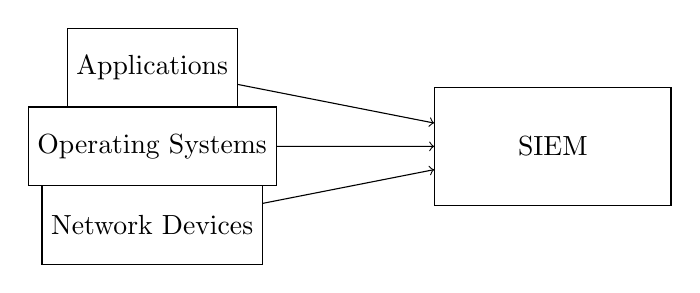
\begin{tikzpicture}[scale = .8]
			\node (apps) [draw, rectangle, minimum width=2cm, minimum height=1cm] {Applications};
			\node (os) [draw, rectangle, minimum width=2cm, minimum height=1cm, below of=apps] {Operating Systems};
			\node (network) [draw, rectangle, minimum width=2cm, minimum height=1cm, below of=os] {Network Devices};
			\node (siem) [draw, rectangle, minimum width=3cm, minimum height=1.5cm, right=2cm of os] {SIEM};
			\draw [->] (apps) -- (siem);
			\draw [->] (os) -- (siem);
			\draw [->] (network) -- (siem);
		\end{tikzpicture}
	\end{frame}
	
	\begin{frame}[fragile]
		\frametitle{3. Time Synchronization: Why Accurate Timestamps Are Critical for Security}
		\begin{itemize}
			\item Time synchronization ensures all devices in a network report events with consistent timestamps.
			\item \textbf{Network Time Protocol (NTP)} is used to synchronize system clocks across a network to a reference time source.
			\item Inconsistent timestamps make it difficult to establish the sequence of events during security incidents.
			\item Time synchronization is essential for correlating events from different systems during an investigation.
		\end{itemize}
		
		\scriptsize
		\begin{semiverbatim}
			# Example of logs with synchronized vs. unsynchronized time
			\alert{Synchronized:}
			2023-10-15 14:32:45 [firewall] Connection blocked from 192.168.1.10
			2023-10-15 14:32:47 [server] Failed login attempt for user admin
			2023-10-15 14:32:48 [IDS] Alert: Possible brute force attack
			
			\alert{Unsynchronized:}
			2023-10-15 14:32:45 [firewall] Connection blocked from 192.168.1.10
			2023-10-15 14:27:12 [server] Failed login attempt for user admin
			2023-10-15 14:39:22 [IDS] Alert: Possible brute force attack
		\end{semiverbatim}
	\end{frame}
	
	\begin{frame}
		\frametitle{4. Understanding Logging Levels: From Debug to Critical}
		\begin{itemize}
			\item \textbf{Logging levels} define the severity and importance of logged events in a system.
			\item Standard logging levels typically include Debug, Info, Warning, Error, and Critical categories.
			\item Higher severity levels (Error, Critical) should trigger immediate alerts for security teams.
			\item Proper configuration of logging levels balances security visibility with storage and processing efficiency.
		\end{itemize}
		
		\begin{table}
			\scriptsize
			\begin{tabular}{|l|l|p{6cm}|}
				\hline
				\textbf{Level} & \textbf{Priority} & \textbf{Description} \\
				\hline
				Debug & Lowest & Detailed information for debugging purposes \\
				\hline
				Info & Low & Normal system operations, successful actions \\
				\hline
				Warning & Medium & Non-critical issues that may require attention \\
				\hline
				Error & High & Runtime errors or unexpected conditions \\
				\hline
				Critical & Highest & System-critical events requiring immediate action \\
				\hline
			\end{tabular}
		\end{table}
	\end{frame}
	
	\begin{frame}
		\frametitle{5. Windows Registry: The Nervous System of Your Operating System}
		\begin{itemize}
			\item The \textbf{Windows Registry} is a hierarchical database that stores configuration settings and options for the operating system.
			\item Registry keys contain critical system and security settings that can be modified by users, applications, or malware.
			\item Security teams monitor registry changes to detect unauthorized modifications or malicious activity.
			\item Improper registry modifications can lead to system instability, security vulnerabilities, or privilege escalation.
		\end{itemize}
		
		\begin{block}{Registry Hives}
			\scriptsize
			\begin{description}
				\item[HKEY\_LOCAL\_MACHINE (HKLM)] System-wide configuration settings
				\item[HKEY\_CURRENT\_USER (HKCU)] Settings specific to the logged-in user
				\item[HKEY\_USERS (HKU)] Settings for all user profiles on the system
				\item[HKEY\_CLASSES\_ROOT (HKCR)] File association and COM object registration
				\item[HKEY\_CURRENT\_CONFIG (HKCC)] Current hardware profile information
			\end{description}
		\end{block}
	\end{frame}
	
	\begin{frame}
		\frametitle{6. System Hardening: Building a Digital Fortress}
		\begin{itemize}
			\item \textbf{System hardening} refers to the process of securing a system by reducing its attack surface and vulnerability exposure.
			\item Hardening involves disabling unnecessary services, closing unused ports, and removing unneeded applications.
			\item Regular security updates and patches are essential components of an effective hardening strategy.
			\item System hardening should be guided by industry-standard benchmarks like CIS (Center for Internet Security) controls.
		\end{itemize}
		
		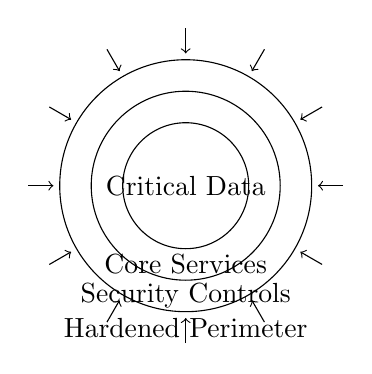
\begin{tikzpicture}[scale = .8]
			\draw (0,0) circle (2cm);
			\draw (0,0) circle (1.5cm);
			\draw (0,0) circle (1cm);
			\node at (0,0) {Critical Data};
			\node at (0,-1.25) {Core Services};
			\node at (0,-1.75) {Security Controls};
			\node at (0,-2.25) {Hardened Perimeter};
			\foreach \angle in {0,30,...,330}
			\draw[->] (\angle:2.5cm) -- (\angle:2.1cm);
		\end{tikzpicture}
	\end{frame}
	
	\begin{frame}
		\frametitle{7. File Structure Fundamentals: Where Your System Stores Critical Data}
		\begin{itemize}
			\item Operating systems organize files in hierarchical structures that determine access permissions and security contexts.
			\item \textbf{File systems} (like NTFS for Windows or ext4 for Linux) implement security features such as access control lists and encryption.
			\item Understanding file structure enables security teams to identify abnormal file placements or unauthorized access attempts.
			\item Critical system files and configurations are stored in protected locations that require elevated privileges to modify.
		\end{itemize}
		
		\begin{example}{Critical Windows File Locations}
			\scriptsize
			\begin{itemize}
				\item \texttt{C:\textbackslash Windows\textbackslash System32} - Core system executables and DLLs
				\item \texttt{C:\textbackslash Windows\textbackslash System32\textbackslash config} - Registry hives
				\item \texttt{C:\textbackslash Windows\textbackslash System32\textbackslash drivers} - Device drivers
				\item \texttt{C:\textbackslash Program Files} - Installed applications (64-bit)
			\end{itemize}
		\end{example}
	\end{frame}
	
	\begin{frame}
		\frametitle{8. Configuration Files: The Security Control Panel of Your System}
		\begin{itemize}
			\item \textbf{Configuration files} store settings that determine how applications and systems operate and handle security.
			\item Security-critical configuration files control authentication, authorization, access control, and encryption settings.
			\item Misconfigurations in these files are a leading cause of security breaches and system vulnerabilities.
			\item Security teams should implement controls for configuration management, version control, and change detection.
		\end{itemize}
		
		\begin{alertblock}{Common Security Misconfigurations}
			Insecure default settings, excessive permissions, hardcoded credentials, unnecessary features enabled, and outdated configuration templates are frequently exploited by attackers to gain unauthorized access.
		\end{alertblock}
	\end{frame}
	
	\begin{frame}[fragile]
		\frametitle{9. System Processes: Identifying Friend from Foe}
		\begin{itemize}
			\item \textbf{System processes} are programs running in memory that perform essential functions for the operating system.
			\item Understanding normal process behavior helps security teams identify anomalous or malicious processes.
			\item Process attributes like parent-child relationships, resource usage, and file access patterns establish behavioral baselines.
			\item Advanced threats often attempt to disguise malicious processes as legitimate system processes.
		\end{itemize}
		
		\scriptsize
		\begin{semiverbatim}
			# Windows Task Manager process list example
			Name               PID   CPU   Memory   User
			System             4     0.1%   0.1 MB   SYSTEM
			smss.exe           372   0.0%   0.7 MB   SYSTEM
			csrss.exe          560   0.2%   3.9 MB   SYSTEM
			wininit.exe        632   0.0%   1.2 MB   SYSTEM
			services.exe       748   0.1%   5.6 MB   SYSTEM
			svchost.exe        856   0.3%  23.4 MB   SYSTEM
			\alert{svchost.exe}      \alert{1345}  \alert{67.2%} \alert{356.8 MB} \alert{SYSTEM}
			explorer.exe      1424   0.5%  45.2 MB   User
		\end{semiverbatim}
	\end{frame}
	
	\begin{frame}
		\frametitle{10. Hardware Architecture Security: From BIOS to Boot Sequence}
		\begin{itemize}
			\item \textbf{Hardware architecture security} involves protecting the physical components and firmware that support computing systems.
			\item The boot sequence represents a critical security phase where systems are vulnerable to low-level attacks.
			\item Secure boot technologies verify the integrity of firmware and boot loaders before the operating system loads.
			\item Hardware-based security features like Trusted Platform Module (TPM) provide cryptographic functions for secure key storage.
		\end{itemize}
		
		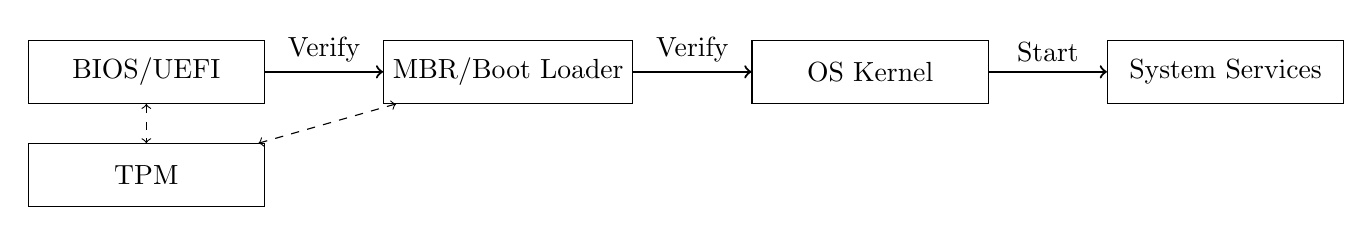
\begin{tikzpicture}[node distance=1.5cm, box/.style={rectangle, draw, minimum width=3cm, minimum height=0.8cm}]
			\node[box] (bios) {BIOS/UEFI};
			\node[box, right=of bios] (mbr) {MBR/Boot Loader};
			\node[box, right=of mbr] (kernel) {OS Kernel};
			\node[box, right=of kernel] (services) {System Services};
			
			\draw[->, thick] (bios) -- node[above] {Verify} (mbr);
			\draw[->, thick] (mbr) -- node[above] {Verify} (kernel);
			\draw[->, thick] (kernel) -- node[above] {Start} (services);
			
			\node[below=0.5cm of bios] (tpm) [box] {TPM};
			\draw[<->, dashed] (bios) -- (tpm);
			\draw[<->, dashed] (mbr) -- (tpm);
		\end{tikzpicture}
	\end{frame}
	
	\begin{frame}
		\frametitle{11. Serverless Security: Protecting Functions in a Cloud-Native World}
		\begin{itemize}
			\item \textbf{Serverless computing} is a cloud execution model where the cloud provider manages infrastructure, allowing developers to focus on code.
			\item The ephemeral nature of serverless functions creates unique security challenges for monitoring and protection.
			\item Security considerations include function permissions, code vulnerabilities, dependency management, and API security.
			\item Traditional security tools designed for persistent infrastructure may not be effective for serverless architectures.
		\end{itemize}
		
		\begin{block}{Serverless Security Challenges}
			\begin{itemize}
				\item Limited execution context makes runtime protection difficult
				\item Shared responsibility model shifts but doesn't eliminate security obligations
				\item Function permissions often follow the principle of least privilege
				\item Third-party dependencies can introduce vulnerabilities
			\end{itemize}
		\end{block}
	\end{frame}
	
	\begin{frame}
		\frametitle{12. Virtualization Security: Isolating Resources Without Isolating Protection}
		\begin{itemize}
			\item \textbf{Virtualization} creates logical instances of computing resources that operate independently on shared physical hardware.
			\item Virtual environments require security controls at both the host and guest levels to prevent cross-VM attacks.
			\item Hypervisor security is critical as compromising this layer could affect all virtual machines under its management.
			\item Virtual network security introduces additional complexity with software-defined networking components.
		\end{itemize}
		
		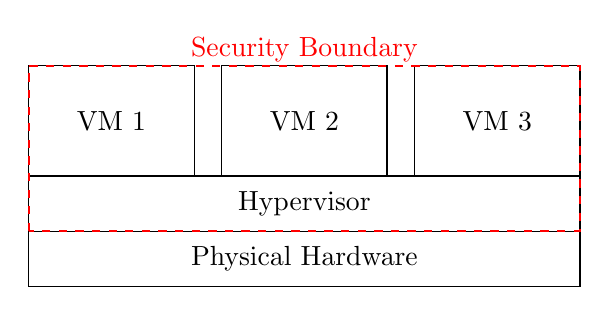
\begin{tikzpicture}[scale = .7]
			\draw (0,0) rectangle (10,1) node[pos=.5] {Physical Hardware};
			\draw (0,1) rectangle (10,2) node[pos=.5] {Hypervisor};
			\draw (0,2) rectangle (3,4) node[pos=.5] {VM 1};
			\draw (3.5,2) rectangle (6.5,4) node[pos=.5] {VM 2};
			\draw (7,2) rectangle (10,4) node[pos=.5] {VM 3};
			\draw[red, thick, dashed] (0,1) rectangle (10,4);
			\node[red] at (5,4.3) {Security Boundary};
		\end{tikzpicture}
	\end{frame}
	
	\begin{frame}
		\frametitle{13. Container Security: Protecting Microservices in Production}
		\begin{itemize}
			\item \textbf{Containers} are lightweight, portable environments that package code and dependencies for consistent operation across environments.
			\item Container security differs from VM security because containers share the host OS kernel, creating a different isolation model.
			\item Security strategies include scanning container images for vulnerabilities, using minimal base images, and implementing runtime protection.
			\item Container orchestration platforms like Kubernetes require additional security considerations for pod communication and secrets management.
		\end{itemize}
		
		\begin{example}{Container Security Best Practices}
			\scriptsize
			\begin{itemize}
				\item Use signed and verified container images from trusted repositories
				\item Implement network policies to control pod-to-pod communications
				\item Apply the principle of least privilege to container runtime permissions
				\item Regularly scan containers for vulnerabilities both pre-deployment and in production
			\end{itemize}
		\end{example}
	\end{frame}
	
	\begin{frame}
		\frametitle{14. On-Premises Architecture: Traditional Security for Traditional Infrastructure}
		\begin{itemize}
			\item \textbf{On-premises architecture} refers to computing resources that are physically located within an organization's facilities.
			\item Traditional security models for on-premises environments often focus on perimeter-based defenses and network segmentation.
			\item Physical security controls complement digital security measures to protect hardware assets and data centers.
			\item On-premises architectures typically provide greater control but require significant capital expenditure and maintenance.
		\end{itemize}
		
		\begin{block}{On-Premises Security Controls}
			\begin{description}
				\item[Physical] Access controls, environmental monitoring, surveillance
				\item[Network] Firewalls, IDS/IPS, network segregation, DMZs
				\item[System] Host hardening, endpoint protection, patch management
				\item[Data] Encryption, access controls, data classification
			\end{description}
		\end{block}
	\end{frame}
	
	\begin{frame}
		\frametitle{15. Cloud Security Architecture: Securing Resources Beyond Your Walls}
		\begin{itemize}
			\item \textbf{Cloud security architecture} addresses the protection of data, applications, and infrastructure hosted by third-party cloud providers.
			\item The shared responsibility model defines security obligations for both cloud providers and customers.
			\item Cloud-native security approaches utilize automation, infrastructure as code, and API-driven controls.
			\item Effective cloud security requires adaptation of traditional security principles to dynamic, scalable environments.
		\end{itemize}
		
	\end{frame}
	\begin{frame}
		\frametitle{Cloud Security Responsibility Matrix}
		\begin{table}[htbp]
			\scriptsize
			\centering
			\caption{Cloud Security Responsibility Matrix}
			\label{tab:cloud_security_responsibility}
			\begin{tabular}{|l|c|c|}
				\hline
				\textbf{Security Aspect} & \textbf{Cloud Provider} & \textbf{Customer} \\ \hline
				Physical Infrastructure Security & \checkmark &  \\ \hline
				Hardware Management & \checkmark &  \\ \hline
				Virtualization Layer & \checkmark &  \\ \hline
				Operating Systems (IaaS) &  & \checkmark \\ \hline
				Operating Systems (PaaS/SaaS) & \checkmark &  \\ \hline
				Application Security (IaaS/PaaS) &  & \checkmark \\ \hline
				Application Security (SaaS) & \checkmark &  \\ \hline
				Identity and Access Management &  & \checkmark \\ \hline
				Data Protection (Encryption at Rest) & \checkmark & \checkmark \\ \hline
				Data Protection (Encryption in Transit) & \checkmark & \checkmark \\ \hline
				Network Security Controls (Infrastructure) & \checkmark &  \\ \hline
				Network Security Controls (User-configured) &  & \checkmark \\ \hline
				Security Monitoring (Infrastructure-level) & \checkmark &  \\ \hline
				Security Monitoring (Application-level) &  & \checkmark \\ \hline
				Compliance (Infrastructure Certifications) & \checkmark &  \\ \hline
				Compliance (Industry-specific Requirements) &  & \checkmark \\ \hline
				Incident Response (Infrastructure-level) & \checkmark &  \\ \hline
				Incident Response (Customer-level) &  & \checkmark \\ \hline
			\end{tabular}
		\end{table}
	\end{frame}
	
	\begin{frame}
		\frametitle{16. Hybrid Infrastructure: Bridging Security Between Worlds}
		\begin{itemize}
			\item \textbf{Hybrid infrastructure} combines on-premises systems with cloud resources, requiring integrated security strategies.
			\item Security challenges include maintaining consistent controls, identity management, and secure connectivity between environments.
			\item Data moving between on-premises and cloud environments must be protected in transit with proper encryption and authorization.
			\item Security monitoring and incident response processes must span both environments for comprehensive protection.
		\end{itemize}
		
		\begin{alertblock}{Hybrid Security Pitfalls}
			Organizations often struggle with security gaps when integrating cloud and on-premises environments, particularly around identity management, access controls, and security visibility across boundaries.
		\end{alertblock}
	\end{frame}
	
	\begin{frame}
		\frametitle{17. Network Segmentation: Building Digital Boundaries That Matter}
		\begin{itemize}
			\item \textbf{Network segmentation} divides a network into multiple segments or subnets, each acting as a security zone with controlled access.
			\item Effective segmentation limits an attacker's lateral movement capabilities following an initial compromise.
			\item Segmentation can be implemented physically (through separate hardware) or logically (using VLANs, firewalls, and ACLs).
			\item The principle of least privilege should guide access controls between network segments.
		\end{itemize}
		
		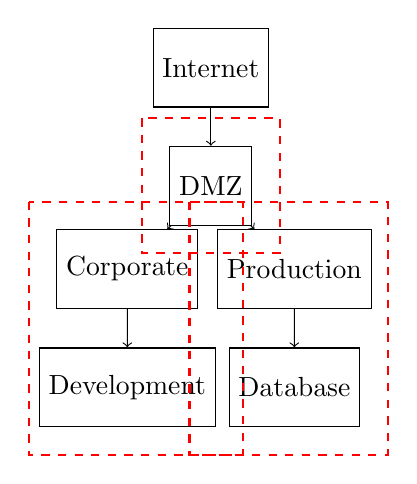
\begin{tikzpicture}[scale = .7, node distance=1.5cm, every node/.style={rectangle, draw, minimum width=1cm, minimum height=1cm}]
			\node (internet) {Internet};
			\node[below of=internet] (dmz) {DMZ};
			\node[below left of=dmz] (corp) {Corporate};
			\node[below right of=dmz] (prod) {Production};
			\node[below of=corp] (dev) {Development};
			\node[below of=prod] (data) {Database};
			
			\draw[->] (internet) -- (dmz);
			\draw[->] (dmz) -- (corp);
			\draw[->] (dmz) -- (prod);
			\draw[->] (corp) -- (dev);
			\draw[->] (prod) -- (data);
			
			\draw[red, thick, dashed] ($(dmz.north west)+(-0.5,0.5)$) rectangle ($(dmz.south east)+(0.5,-0.5)$);
			\draw[red, thick, dashed] ($(corp.north west)+(-0.5,0.5)$) rectangle ($(dev.south east)+(0.5,-0.5)$);
			\draw[red, thick, dashed] ($(prod.north west)+(-0.5,0.5)$) rectangle ($(data.south east)+(0.5,-0.5)$);
		\end{tikzpicture}
	\end{frame}
	
	\begin{frame}
		\frametitle{18. Zero Trust Architecture: Never Trust, Always Verify}
		\begin{itemize}
			\item \textbf{Zero Trust} is a security model that assumes no user or system should be inherently trusted, regardless of location or network.
			\item Zero Trust principles include verifying identity, validating device health, enforcing least privilege, and assuming breach.
			\item Implementation requires strong identity management, micro-segmentation, and continuous monitoring and validation.
			\item Zero Trust represents a shift from perimeter-based security to identity and data-centric approaches.
		\end{itemize}
		
		\begin{block}{Zero Trust Core Principles}
			\scriptsize
			\begin{enumerate}
				\item Verify explicitly - Always authenticate and authorize based on all available data points
				\item Use least privileged access - Limit user access with Just-In-Time and Just-Enough-Access
				\item Assume breach - Minimize blast radius and segment access, verify end-to-end encryption
				\item Apply behavioral analytics to detect anomalies in real-time
			\end{enumerate}
		\end{block}
	\end{frame}
	
	\begin{frame}
		\frametitle{19. Secure Access Service Edge (SASE): Converging Network and Security in the Cloud Era}
		\begin{itemize}
			\item \textbf{Secure Access Service Edge (SASE)} combines network security functions with WAN capabilities to support secure access for distributed organizations.
			\item SASE delivers security controls as cloud-based services, closer to the users and devices that need them.
			\item Core components include SD-WAN, Secure Web Gateway, CASB, Zero Trust Network Access, and FWaaS.
			\item SASE addresses the challenge of securing remote workforces and cloud applications beyond traditional network boundaries.
		\end{itemize}
		
		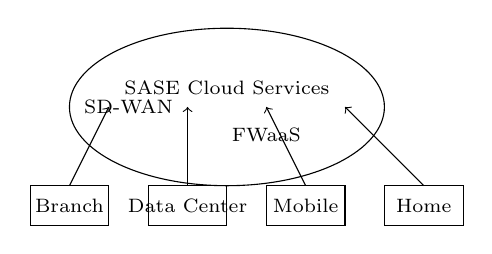
\begin{tikzpicture}[scale = .5]
			\scriptsize
			\draw (0,0) ellipse (4cm and 2cm);
			\node at (0,.5) {SASE Cloud Services};
			\node at (-2.5,0) {SD-WAN};
			\node at (1,-0.7) {FWaaS};
			
			\draw (-5,-3) rectangle (-3,-2) node[pos=.5] {Branch};
			\draw (-2,-3) rectangle (0,-2) node[pos=.5] {Data Center};
			\draw (1,-3) rectangle (3,-2) node[pos=.5] {Mobile};
			\draw (4,-3) rectangle (6,-2) node[pos=.5] {Home};
			
			\draw[->] (-4,-2) -- (-3,0);
			\draw[->] (-1,-2) -- (-1,0);
			\draw[->] (2,-2) -- (1,0);
			\draw[->] (5,-2) -- (3,0);
		\end{tikzpicture}
	\end{frame}
	
	\begin{frame}
		\frametitle{20. Software-Defined Networking: Security in a Programmable Network}
		\begin{itemize}
			\item \textbf{Software-Defined Networking (SDN)} separates the network control plane from the data plane, enabling programmatic network management.
			\item SDN enhances security through centralized policy enforcement, dynamic network segmentation, and automated threat response.
			\item The SDN controller becomes a critical security component that must be protected from unauthorized access or manipulation.
			\item Security benefits include improved visibility, consistent policy application, and rapid response to detected threats.
		\end{itemize}
		
		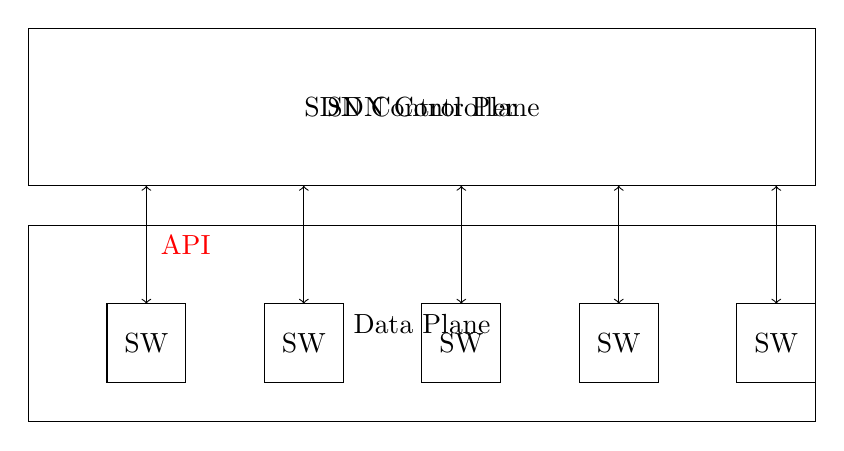
\begin{tikzpicture}
			\draw (0,3) rectangle (10,5) node[pos=.5] {SDN Control Plane};
			\draw[dashed] (0,3) -- (10,3);
			\draw (0,0) rectangle (10,2.5) node[pos=.5] {Data Plane};
			
			\node at (5,4) {SDN Controller};
			\draw (1,0.5) rectangle (2,1.5) node[pos=.5] {SW};
			\draw (3,0.5) rectangle (4,1.5) node[pos=.5] {SW};
			\draw (5,0.5) rectangle (6,1.5) node[pos=.5] {SW};
			\draw (7,0.5) rectangle (8,1.5) node[pos=.5] {SW};
			\draw (9,0.5) rectangle (10,1.5) node[pos=.5] {SW};
			
			\draw[<->] (1.5,1.5) -- (1.5,3);
			\draw[<->] (3.5,1.5) -- (3.5,3);
			\draw[<->] (5.5,1.5) -- (5.5,3);
			\draw[<->] (7.5,1.5) -- (7.5,3);
			\draw[<->] (9.5,1.5) -- (9.5,3);
			
			\node[red] at (2,2.25) {API};
		\end{tikzpicture}
	\end{frame}
	
	\begin{frame}
		\frametitle{24. Federation: Managing Identity Across Organizational Boundaries}
		\begin{itemize}
			\item \textbf{Federation} is a mechanism that enables separate organizations to share identity information securely across trust boundaries.
			\item Federated identity allows users to use credentials from one domain to access resources in another domain without creating multiple accounts.
			\item Federation relies on established trust relationships between identity providers and service providers.
			\item Implementation typically uses standards like SAML, WS-Federation, or OAuth/OpenID Connect to securely exchange identity assertions.
		\end{itemize}
		
		\begin{example}{Federation in Action}
			A university professor can use their university credentials (identity provider) to access an external research database (service provider) without creating a separate account. The research database trusts the university to properly authenticate the professor, while the university maintains control over the professor's authentication methods and access rights.
		\end{example}
	\end{frame}
	
	\begin{frame}
		\frametitle{21. Identity: The New Security Perimeter}
		\begin{itemize}
			\item \textbf{Identity} has become the primary security boundary in modern environments where traditional network perimeters are dissolving.
			\item Identity and access management (IAM) systems provide the foundation for authenticating users and authorizing access to resources.
			\item Identity-focused security requires continuous validation of user identity, device health, and contextual risk factors.
			\item Identity systems must be protected as critical infrastructure since compromise can lead to widespread access across environments.
		\end{itemize}
		
		\begin{alertblock}{Identity as the Attack Vector}
			\scriptsize
			Compromised credentials are involved in over 80\% of data breaches, making identity protection a critical security priority. Attack techniques like password spraying, credential stuffing, and phishing specifically target this new perimeter.
		\end{alertblock}
	\end{frame}
	
	\begin{frame}
		\frametitle{22. Multifactor Authentication: Why Passwords Alone Are Not Enough}
		\begin{itemize}
			\item \textbf{Multifactor Authentication (MFA)} requires two or more verification factors: something you know, something you have, or something you are.
			\item MFA significantly reduces the risk of account compromise, even when passwords are leaked or stolen.
			\item Authentication factors vary in security strength, with biometrics and hardware tokens generally offering stronger protection than SMS codes.
			\item Proper MFA implementation requires balancing security requirements with user experience considerations.
		\end{itemize}
		
		\begin{table}
			\scriptsize
			\begin{tabular}{|l|l|l|}
				\hline
				\textbf{Factor Type} & \textbf{Examples} & \textbf{Security Level} \\
				\hline
				Knowledge & Passwords, PINs, Security questions & Low-Medium \\
				\hline
				Possession & Hardware tokens, Mobile apps, Smart cards & Medium-High \\
				\hline
				Inherence & Fingerprints, Facial recognition, Voice & High \\
				\hline
				Location & GPS, Network location & Medium \\
				\hline
				Behavior & Typing patterns, Usage patterns & Medium \\
				\hline
			\end{tabular}
		\end{table}
	\end{frame}
	
	\begin{frame}
		\frametitle{23. Single Sign-On: Balancing Security and User Experience}
		\begin{itemize}
			\item \textbf{Single Sign-On (SSO)} allows users to authenticate once and gain access to multiple applications without additional login prompts.
			\item SSO improves security by reducing password fatigue, enabling centralized authentication management, and streamlining access revocation.
			\item SSO implementations typically use protocols like SAML, OAuth, or OpenID Connect to securely share authentication information.
			\item While SSO creates a single point of entry, it should be strengthened with MFA and continuous monitoring to mitigate this risk.
		\end{itemize}
		
=
		\end{frame}
\end{document}